\documentclass{beamer}

\usetheme{Darmstadt}
\usecolortheme{crane}

\usepackage[T1]{fontenc}
\usepackage{eurosym}
\usepackage{lmodern}
\usepackage[utf8]{inputenc}
\usepackage[french]{babel}

\addtobeamertemplate{footline}{ ~\insertframenumber / \inserttotalframenumber}

\title{Frameworks de développement cross-platform}
\subtitle{L'avenir du développement mobile ?}
\author{Thibaud Destouches \& Marceau Lacroix}
\date{}
\institute{ISTIC -- Université de Rennes 1}

\begin{document}

\begin{frame}[fragile]
\titlepage
\end{frame}

\begin{frame}
\setcounter{tocdepth}{2}
\tableofcontents
\end{frame}

\section{Introduction}
\subsection{Problématique}

\begin{frame}
  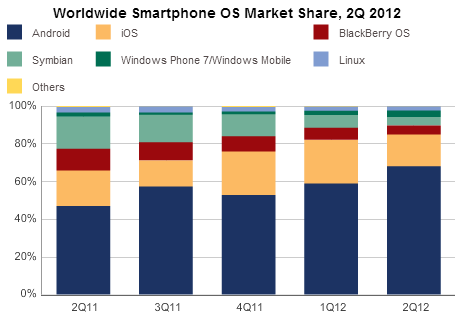
\includegraphics[scale=0.9]{segm}
\end{frame}

\begin{frame}{Solution}
\begin{center}
  Une solution ?
  \\ ~ \\
  \textbf{Frameworks de développement cross-platform mobile}
\end{center}
\end{frame}

\subsection{Enjeux}
\begin{frame}
\textbf{Un secteur en grande progression...}
\\ ~ \\
  \begin{itemize}
    \item Profiter d'un marché de plus en plus importants
    \begin{itemize}
      \item Ventes Smartphones > Ventes PC (2012)
    \end{itemize}
    \item Réduire le Time-to-Market
    \item Limiter la segmentation des OS
    \begin{itemize}
      \item Android (68.1 \%)
      \item iOS (16.9 \%)
      \item BlackBerry OS (4.8 \%)
      \item Windows Phone (4.4 \%)
      \item ...
    \end{itemize}
    \item Faciliter la maintenabilité
  \end{itemize}
\end{frame}


\section{Etat de l'art}
\begin{frame}
\setcounter{tocdepth}{2}
\tableofcontents[currentsection]
\end{frame}

\subsection{Compilation Web}
\begin{frame}
\begin{columns}[c]
  \begin{column}{0.5\textwidth}
    \begin{center}
      
\includegraphics[scale=0.3]{sencha}
    \end{center}
  \end{column}
  \begin{column}{0.5\textwidth}
    \begin{itemize}
      \item Requiert uniquement des connaissance en HTML/JavaScript.
\item Faibles performances.
\item Pas d'accès au materiel.
    \end{itemize}
  \end{column}
\end{columns}
\end{frame}

\subsection{Compilation hybride}
\begin{frame}
\begin{columns}[c]
  \begin{column}{0.5\textwidth}
    \begin{itemize}
      \item Requiert l'apprentissage d'un DSL ou d'APIs.
	\item Performances correctes.
	\item accès au materiel courant (GPS, Contacts, accéléromètre, ...)
    \end{itemize}
  \end{column}
  \begin{column}{0.5\textwidth}
    \begin{center}
      
\includegraphics[scale=0.4]{titanium} \\
	\textbf{Titanium, PhoneGap, Rhodes}
    \end{center}
  \end{column}
\end{columns}
\end{frame}

\subsection{Compilation native}
\begin{frame}
\begin{columns}[c]
  \begin{column}{0.5\textwidth}
    
\includegraphics[scale=0.7]{corona}
\textbf{Corona}
  \end{column}
  \begin{column}{0.5\textwidth}
    \begin{itemize}
\item Requiert l'apprentissage d'un DSL.
      \item Performances élevées.
\item Emploi pour une utilisation  spécifique.
    \end{itemize}
  \end{column}
\end{columns}
\end{frame}

\subsection{Voind}
\begin{frame}
\begin{columns}[c]
  \begin{column}{0.5\textwidth}
    \begin{itemize}
      \item Requiert l'apprentissage d'un DSL.
	\item Performances élevées.
	\item accès au materiel total.
\item requiert des connaissances sur chaque plateforme
\item peu de code généré (50\%)
    \end{itemize}
  \end{column}
  \begin{column}{0.5\textwidth}
    \begin{center}
      
\includegraphics[scale=0.4]{voind} \\
	\textbf{Voind}, pas vraiment un un framework cross-platform
    \end{center}
  \end{column}
\end{columns}
\end{frame}

\section{Conclusion}
\begin{frame}
\setcounter{tocdepth}{2}
\tableofcontents[currentsection]
\end{frame}


\subsection{Avantages / Inconvénients}
\begin{frame}
\begin{columns}[c]
  \begin{column}{0.5\textwidth}
    \textbf{Avantages}
    \begin{itemize}
      \item Réduction du temps de développement
      \item Maintenabilité facilité
    \end{itemize}
  \end{column}
  \begin{column}{0.5\textwidth}
    \textbf{Inconvénients}
    \begin{itemize}
      \item Limitation des APIs
      \item Compilation Web
      \item Code généré de qualité inférieur à un développement spécifique
      \item Non support de certains matériels
      \item Prix de la licence
    \end{itemize}
  \end{column}
\end{columns}
\end{frame}

\subsection{Conclusion}
\begin{frame}
\begin{center}
  \textbf{Ces Frameworks sont-ils viables ?}
  \\ ~ \\ ~
  \textbf{Pour quels besoins ?}
  \\ ~ \\ ~
  \textbf{A quel coûts ?}
\end{center}
\end{frame}

\subsection{Bibliographie}
\begin{frame}
\begin{thebibliography}{9}
   \bibitem{timo11}
          Timo Paananen,
          \emph{Smartphone Cross-Plaform Frameworks}.
          Jamk University of Applied Sciences,
          avril 2011.
   \bibitem{bruning11}
          Mathieu Bruning,
          \emph{Native Cross-Platform Mobile Application Development Using Voind}.
          Faculty EEMCS, Delft University of Technology,
          novembre 2011.
   \bibitem{appcreator}
          Appcelerator Inc,
          \emph{http://www.appcelerator.com/}.
   \bibitem{rhomobile}
          Rhomobile Suite,
          \emph{http://www.motorola.com/}.
   \bibitem{phonegap}
          PhoneGap,
          \emph{http://phonegap.com/}.
   \bibitem{phonegap}
          Sencha,
          \emph{http://www.sencha.com/products/touch/}.
   \bibitem{corona}
          Corona,
          \emph{http://www.coronalabs.com/}.
\end{thebibliography}
\end{frame}

\begin{frame}{Questions}
\begin{center}
  Merci de votre attention.
  \\ ~ \\ ~
  \textbf{Avez-vous des questions ?}
\end{center}
\end{frame}


\end{document}
